\section{Run-Time Analysis}\label{sec:run_time}

Both the Python and Rust versions of the algorithm were tested comparatively through a structured benchmarking experiment, with the goal of analyzing the similarity in empirical time complexity and solution quality between both implementations across different seeds and input networks. For both code versions, wall-clock timing was recorded for algorithm initialization times (the process of randomly generating an initial solution) and for a 50-generation run, including initialization times. These timings were repeated 15 times per seed, including one discarded ‘warmup round’ to ensure measurements reflect steady-state performance rather than initial overheads. 6 seeds were tested on both implementations, allowing for matched observations and paired analysis between versions with sufficient statistical power. For each seed-version pair, the mean completion time, time per generation, and mean speedup was derived through individual trial data. Time per generation was calculated by subtracting a seed’s mean initialization time from the recorded full time and dividing by 50. The outlined timing experiment was conducted on the Unitrans and SFMTA networks. 

It should be noted that the Rust implementation utilizes multi-threaded parallelism via Rayon for the solution solving task, as opposed to Python’s single-threaded execution. Though theoretically feasible, parallel execution was not considered for the Python implementation due to non-negligible overhead from object serialization across process boundaries. Rayon uses all available logical cores by default, with hardware specifications reported in Table \ref{tab:computer_specs}. The core NSGA-II algorithm is otherwise identical across both implementations and takes the same network input and other hyperparameters as the Python version, relying on PyO3 to provide the Rust bindings for the Python interpreter and Maturin to compile the Rust code and build a standard Python wheel for distribution. This implementation allows for the Rust backend to be utilized directly from a Python environment as a standard importable module, requiring no changes to the existing user-facing interface or practical workflow.

\begin{table}[H]
	\caption{Specifications of computer used for run-time experiment}
	\label{tab:computer_specs}
	\begin{tabular}{|C{.5\linewidth}|C{.5\linewidth}|}
		\hline Component & Specification \\
		\hline CPU & Apple M2 \\
		\hline Core configuration & 8 cores (4 performance + 4 efficiency) \\
		\hline Memory & 16 GB unified memory \\
		\hline L1 cache (I/D) & 128 KB/64 KB \\
		\hline L2 cache & 4 MB \\
		\hline L3 cache & Not present (Apple Silicon uses unified L2) \\
		\hline Clock speed & 3.49 GHz \\
		\hline              
	\end{tabular}
\end{table}

Rust compilation flags include opt-level=3, lto=true, and codegen-units=1. No CPU affinity pinning or process isolation was applied. The OS scheduler was free to migrate threads across all 8 cores. In addition to hardware and software specifications, both the Python and Rust versions of the algorithm were evaluated with the hyperparameters described in Table \ref{tab:hyperparameters}. For timing analysis, Unitrans and SFMTA utilized the same hyperparameters, whereas network-specific hyperparameters were utilized for convergence comparison.

\begin{table}[H]
	\caption{Hyperparameters used for run-time experiment}
	\label{tab:hyperparameters}
	\begin{tabular}{|C{.25\linewidth}|C{.25\linewidth}|C{.25\linewidth}|C{.25\linewidth}|}
		\hline Hyperparameter & \multicolumn{1}{c|}{Timing comparison} & \multicolumn{2}{c|}{Convergence comparison} \\
		\hline &  & Unitrans & SFMTA \\
		\hline Maximum iterations & 50 & 600 & 1000 \\
		\hline Initialization population size & 100 & 500 & 1500 \\
		\hline Core population size & 100 & 150 & 200 \\
		\hline Mutation probability & 0.15 & 0.15 & 0.15 \\
		\hline Crossover probability & 0.5 & 0.5 & 0.75 \\
		\hline Survival threshold & 0 & 0 & 0 \\
		\hline Retries & 50 & 3 & 3 \\
		\hline
	\end{tabular}
\end{table}

\subsection{Timing Results}

The per-network results are given for each seed implementation pair in Tables \ref{tab:timing_unitrans} and \ref{tab:timing_sfmta}. The Shapiro-Wilk test was conducted on each sample to assess the normality of timing distributions, resulting in several statistically significant p-values. This indicates that timing distributions were not consistently normally distributed across trials, which is expected, as timing distributions for iterative algorithms are often right-skewed \cite{Gomes_2000_JAR}. Because of this, non-parametric techniques such as Bootstrapped \glspl{ci} and the Wilcoxon signed-rank test were used for subsequent statistical analysis, as they do not make assumptions about the underlying data distribution. The Wilcoxon signed-rank test was chosen to analyze paired Python-Rust timings for statistically significant differences. A 95\% \gls{ci} with 9,999 resamples was utilized for all intervals constructed, and all bootstrap resampling was completed with the same random state. A statistically significant time performance difference was found between the Python and Rust implementations for the initialization and full runs of the Unitrans and SFMTA networks

\begin{table}[H]
	\caption{Run-time results for Unitrans example network}
	\label{tab:timing_unitrans}
	\begin{tabular}{|C{.1428\linewidth}|C{.1428\linewidth}|C{.1428\linewidth}|C{.1428\linewidth}|C{.1428\linewidth}|C{.1428\linewidth}|C{.1428\linewidth}|}
		\hline \multicolumn{1}{|c|}{Seed} & \multicolumn{2}{c|}{Initialization (s)} & \multicolumn{2}{c|}{Full Run (s)} & \multicolumn{2}{c|}{Time/Generation (s)} \\
		\hline Language & Python & Rust & Python & Rust & Python & Rust \\
		\hline 0 & 3.332 (0.035) & 0.183 (0.0007) & 94.39 (0.138) & 4.203 (0.019) & 1.821 & 0.080 \\
		\hline 1 & 3.316 (0.051) & 0.185 (0.004) & 93.05 (0.084) & 4.216 (0.017) & 1.795 & 0.081 \\
		\hline 2 & 3.313 (0.033) & 0.185 (0.001) & 91.83 (0.410) & 4.216 (0.051) & 1.770 & 0.082 \\
		\hline 3 & 3.445 (0251) & 0.185 (0.008) & 94.45 (0.215) & 4.201 (0.027) & 1.820 & 0.080 \\
		\hline 4 & 3.337 (0.032) & 0.184 (0.001) & 93.75 (0.141) & 4.287 (0.027) & 1.808 & 0.082 \\
		\hline 5 & 3.317 (0.064) & 0.183 (0.002) & 93.66 (0.130) & 4.260 (0.042) & 1.807 & 0.082 \\
		\hline
	\end{tabular}
\end{table}

\begin{table}[H]
	\caption{Run-time results for SFMTA example network}
	\label{tab:timing_sfmta}
	\begin{tabular}{|C{.1428\linewidth}|C{.1428\linewidth}|C{.1428\linewidth}|C{.1428\linewidth}|C{.1428\linewidth}|C{.1428\linewidth}|C{.1428\linewidth}|}
		\hline \multicolumn{1}{|c|}{Seed} & \multicolumn{2}{c|}{Initialization (s)} & \multicolumn{2}{c|}{Full Run (s)} & \multicolumn{2}{c|}{Time/Generation (s)} \\
		\hline Language & Python & Rust & Python & Rust & Python & Rust \\
		\hline 0 & 14.49 (0.083) & 0.628 (0.008) & 483.2 (0.462) & 24.59 (0.088) & 9.374 & 0.479 \\
		\hline 1 & 14.52 (0.101) & 0.632 (0.008) & 486.3 (0.497) & 24.83 (0.073) & 9.435 & 0.484 \\
		\hline 2 & 14.55 (0.052) & 0.622 (0.006) & 489.2 (0.537) & 25.14 (0.103) & 9.494 & 0.490 \\
		\hline 3 & 14.55 (0.161) & 0.620 (0.011) & 486.9 (2.844) & 25.25 (0.095) & 9.447 & 0.493 \\
		\hline 4 & 14.50 (0.062) & 0.626 (0.006) & 486.2 (0.450) & 25.14 (0.110) & 9.434 & 0.490 \\
		\hline 5 & 14.51 (0.051) & 0.630 (0.005) & 488.9 (1.766) & 25.03 (0.323) & 9.488 & 0.488 \\
		\hline
	\end{tabular}
\end{table}

\subsection{Convergence Comparison}

Convergence quality was assessed using the hypervolume indicator, which is defined as the volume of objective space dominated by the Pareto front and bounded by a reference point set to 110\% of the worst observed objective values across all runs. A higher hypervolume indicates a larger, better-spread front. Paired hypervolumes across seeds was evaluated for both the Unitrans and SFMTA networks to compare the rate, quality, and similarity of convergence across implementations. For convergence testing, the max_iter hyperparameter was set to 600 for Unitrans, and 1,000 for SFMTA. Convergence was determined via the retries parameter, which was set to 3. The retries parameter terminates the evolution process early if no updates to the chosen population are made within a certain number of attempts. Figure \ref{fig:hypervolume_convergence} highlights the convergence via hypervolume for Python and Rust implementations across all seeds, showing mean hypervolume per generation $\pm 1$ standard deviation. Average hypervolume remains similar over generations, indicating consistency across algorithms. All solutions ran to convergence.

\begin{figure}[H]
	\centering
	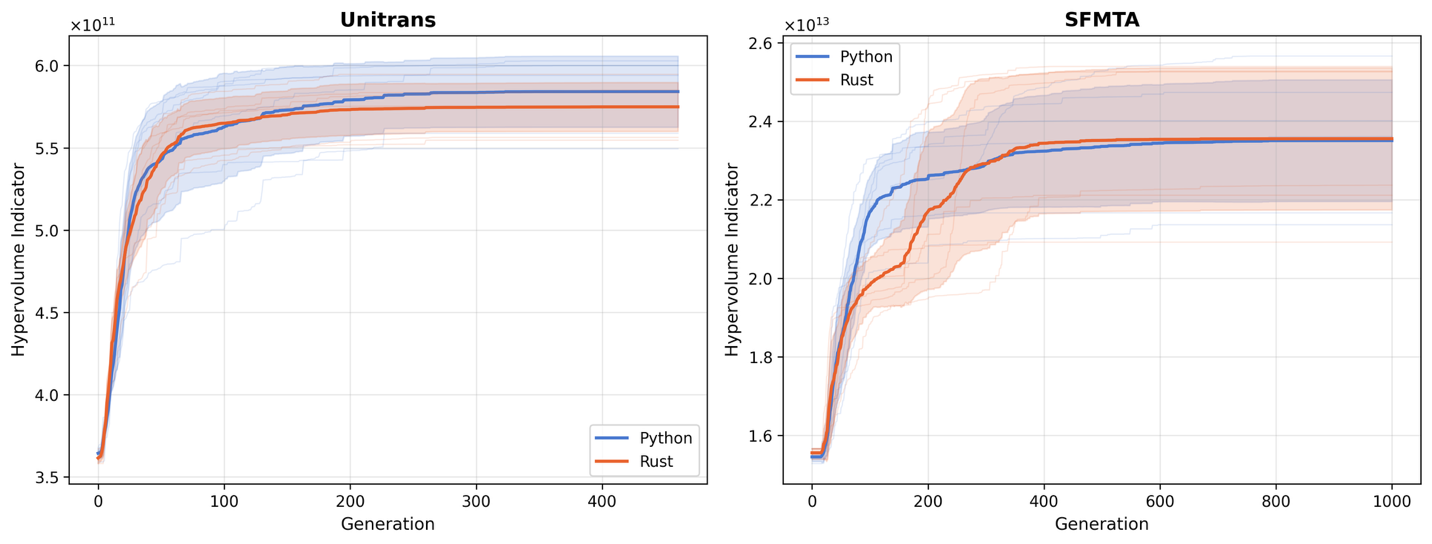
\includegraphics[width = \linewidth]{./figs/hypervolume_convergence.png}
	\caption{Evolution of hypervolume by generation for Python and Rust implementations for Unitrans and SFMTA networks.}
	\label{fig:hypervolume_convergence}
\end{figure}

Two Wilcoxon signed-rank tests were conducted on the paired Python-Rust hypervolumes for Unitrans and SFMTA, with p-values of 0.5625 and 1.0000, respectively. These results are displayed in Figure \ref{fig:hypervolume_boxplots}. This indicates that there is no statistically significant difference between the hypervolumes produced across seeds in either implementation.


\begin{figure}[H]
	\centering
	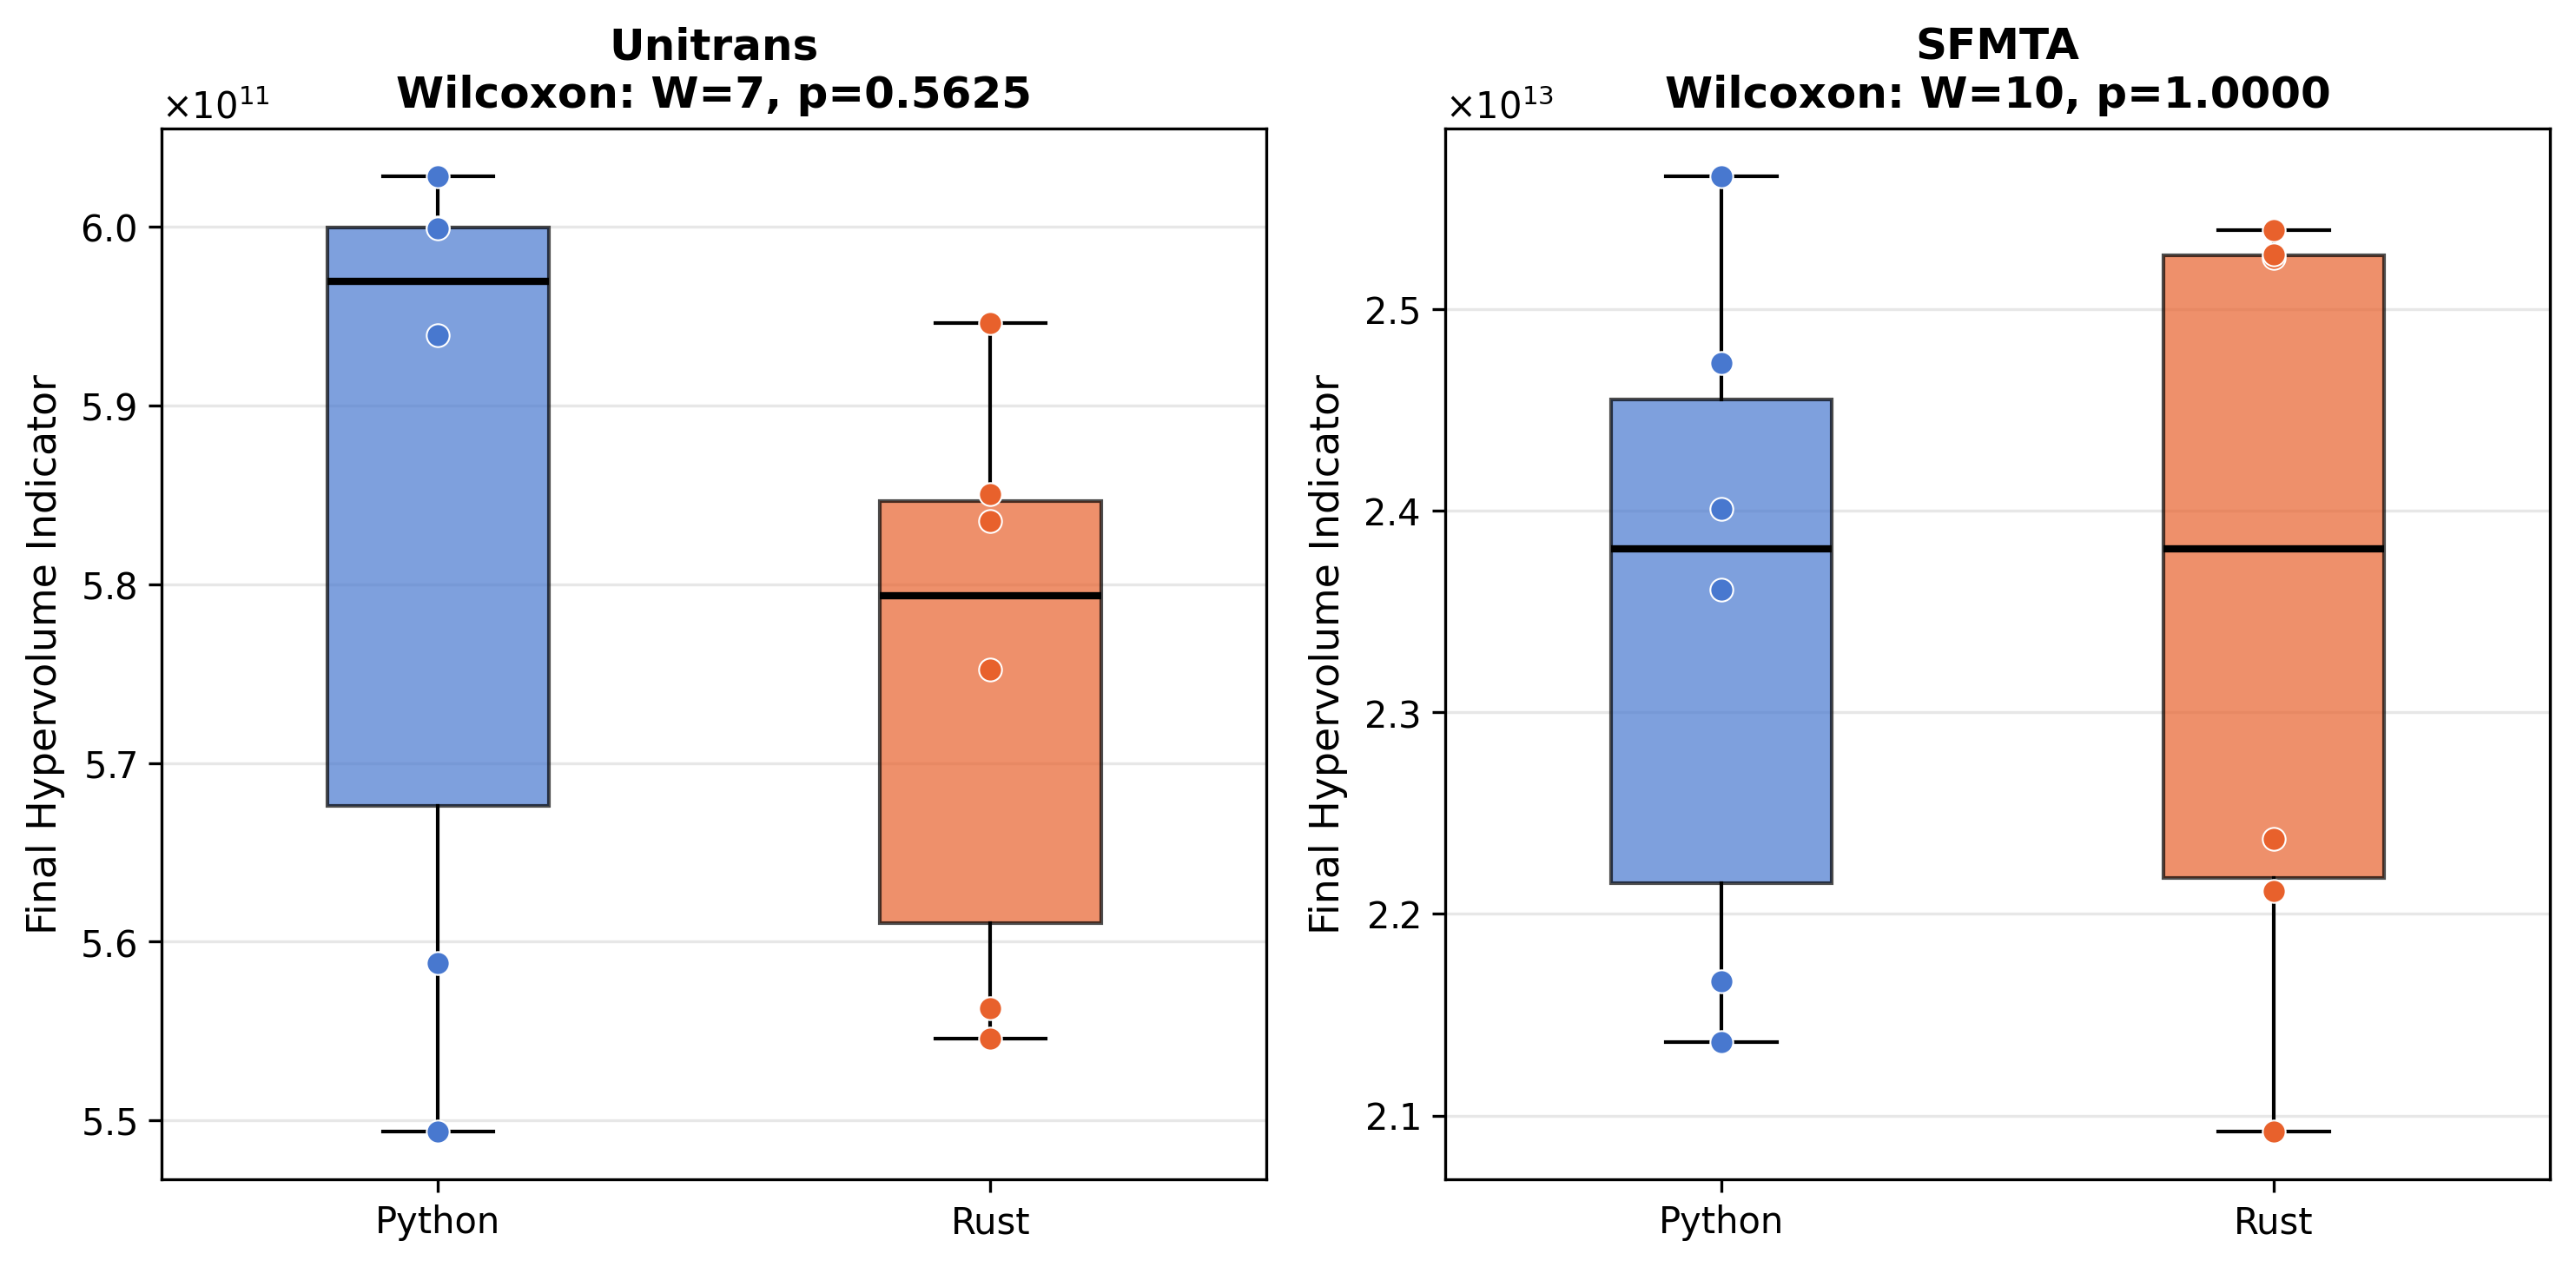
\includegraphics[width = \linewidth]{./figs/hypervolume_boxplots.png}
	\caption{Boxplots of final hypervolume for Python and Rust implementations for Unitrans and SFMTA networks.}
	\label{fig:hypervolume_boxplots}
\end{figure}